\section{$\gamma$ 形状模与取向模的耦合}\label{sec:3-6}

在非轴对称变形核的集体激发谱学中，摆动运动（wobbling motion）与 $\gamma$ 振动对应不同的局域自由度。前者描述角动量相对于内禀主轴的小幅取向运动（取向模）；后者描述四极形状参数 $\gamma$ 在选定平衡形状附近的变化（形状模），平衡点本身可以具有非零 $\gamma$。一个容易理解的区别是：取向运动改变椭球怎样转，形状运动改变椭球各轴怎样伸缩。冻结形状的转子模型只保留前一类自由度；把两类运动同时纳入后，还需检查它们是否能够近似分离。

然而，第\ref{chap:2}章第\ref{sec:2-6}节建立的微观动能响应分析表明，核体系的三轴转动惯量并非外生给定的几何常数，而是单粒子运动与残余配对相互作用在随体参考系中自洽极化的动态产物；同时，第\ref{sec:3-2}节指出稳定转轴的选择严格依赖于角速度与惯量排布的动力学平衡。随着转动自旋增加，科里奥利力与离心力引发强烈的微观形状极化，内禀势能曲面的形状刚度随之演化，使得取向振动模与形状振动模的特征能标可能在特定自旋区间相互接近。本节的核心任务是探讨这两类自由度发生动力学耦合的物理条件：从双自由度局域正规模教学模型出发，阐述避免交叉与跃迁强度交换的联合预言判据；分析推转自洽响应中旋转 Nambu--Goldstone 模与转动赝模的微观剔除；澄清有限自旋非谐性与局域声子标签的适用界限；并结合微观模型案例与实验测量，评估这一模式耦合的实际辨识边界。\cite{prochniak-rohozinski-2009-bohr-collective-hamiltonian,matsuzaki-2004-nuclear-inertia-and-wobbling,kvasil-2006-dy156-yb162-crpa-wobbling,doctoral-r1-g37-oi-2001-wobbling-gamma-coupling,doctoral-r1-g37-bhat-2025-microscopic-wobbling-even-even}

\subsection{双坐标耦合的正规模教学模型}\label{sec:3-6-1}

为了在简明物理框架下展示形状偏离与取向进动的微振动耦合本构，本小节构建一个包含两个声明局域广义坐标的正则耦合振子模型。为了避免与四极形状不变量 $q_2, q_3$ 产生记号冲突，令标量坐标 $\xi_1$ 代表内禀形状参数偏离自洽极小的无量纲局域位移（形状模），标量坐标 $\xi_2$ 代表转动角动量矢量偏离主惯量转轴的小振幅角偏离（取向模）；$p_{\xi_1}$ 与 $p_{\xi_2}$ 分别为其共轭动量，满足标准正则对易关系 $[\xi_i, p_{\xi_j}] = i\hbar\delta_{ij}$。

在选定势阱极小邻域内，将动能与势能截断至二次项，构造局域有效哈密顿量：
\begin{equation}\label{eq:3-6-two-coord-hamiltonian}
H_{\mathrm{local}} = \left(\frac{p_{\xi_1}^2}{2B_1} + \frac{p_{\xi_2}^2}{2B_2}\right) + \frac{1}{2} C_1 \xi_1^2 + \frac{1}{2} C_2 \xi_2^2 + C_{12} \xi_1 \xi_2 ,
\end{equation}
其中质量参数 $B_1, B_2 > 0$；$C_1, C_2$ 分别为两模式的非耦合弹性恢复刚度系数，交叉刚度项 $C_{12}$ 表征形状偏离对空间取向力矩的线性微扰耦合。为了保证局域极小的动力学稳定性，势能二次型刚度矩阵：
\begin{equation}\label{eq:3-6-stiffness-matrix}
\mathbf{C} = \begin{pmatrix} C_1 & C_{12} \\ C_{12} & C_2 \end{pmatrix}
\end{equation}
必须满足正定性条件，即：
\begin{equation}\label{eq:3-6-positive-definite}
C_1 > 0, \quad C_2 > 0, \quad \det\mathbf{C} = C_1 C_2 - C_{12}^2 > 0 \implies C_{12}^2 < C_1 C_2 .
\end{equation}
条件\eqref{eq:3-6-positive-definite}保证两支谐振频率为正。当 $C_{12}^2=C_1C_2$ 时，一支频率降到零，二次近似不能决定该方向的恢复力；若进一步使行列式为负，则出现负曲率方向，原展开点失稳。零频附近需要检查高阶势能项。

引入质量加权坐标 $x_i = \sqrt{B_i}\,\xi_i$ 与未耦合角频率 $\omega_1 = \sqrt{C_1/B_1}$、$\omega_2 = \sqrt{C_2/B_2}$，系统运动方程可转化为对称动力学矩阵的本征值问题。因为 $\xi_i$ 无量纲，$B_i$ 的量纲为能量乘时间平方，$C_i$ 为能量，以下矩阵的量纲是时间的负二次方：
\begin{equation}\label{eq:3-6-dynamic-matrix}
\mathbf{M} = \mathbf{B}^{-1/2} \mathbf{C} \mathbf{B}^{-1/2} = \begin{pmatrix} \omega_1^2 & \dfrac{C_{12}}{\sqrt{B_1 B_2}} \\ \dfrac{C_{12}}{\sqrt{B_1 B_2}} & \omega_2^2 \end{pmatrix} .
\end{equation}
对角化矩阵 $\mathbf{M}$，即可解出耦合体系的两支正规模特征固有频率 $\omega_\pm$：
\begin{equation}\label{eq:3-6-eigenfrequencies}
\omega_\pm^2 = \frac{1}{2}\left(\omega_1^2 + \omega_2^2 \pm \sqrt{(\omega_1^2 - \omega_2^2)^2 + 4 \frac{C_{12}^2}{B_1 B_2}}\right) .
\end{equation}
式\eqref{eq:3-6-eigenfrequencies}表明：只要交叉耦合项 $C_{12} \neq 0$，两支频率便不简并。在未耦合频率相等（$\omega_1 = \omega_2$）处，频率平方差为：
\begin{equation}\label{eq:3-6-min-gap}
\Delta(\omega^2)\big|_{\mathrm{res}} = \omega_+^2 - \omega_-^2 = \frac{2 |C_{12}|}{\sqrt{B_1 B_2}} .
\end{equation}
需要指出，式\eqref{eq:3-6-two-coord-hamiltonian}至\eqref{eq:3-6-min-gap}是在常质量与常恢复力下的正则教学振动模型，尚未包含推转旋转体系中普遍存在的科氏陀螺速度依赖耦合项（gyro-coupling），不宣称其为微观 QRPA 响应方程的精确约化，亦不能将该模型的局域参数拟合等同于对实际核多体系统的直接实测。

\subsection{量子两态混合的对称性与相互作用条件}\label{sec:3-6-2}

当从经典局域微振动推进至量子多体能态表述时，形状振动与取向摆动的模式耦合表现为具有确定实验室量子数的离散态之间的组态混合。

设原子核在特定自旋 $I_i$ 下存在两个未微扰的正交基底态：未微扰的纯 $\gamma$ 振动态 $|1\rangle \equiv |I_i, \gamma\text{-vib}\rangle$（未耦合能量为 $\varepsilon_1^{(0)}$）与纯取向摆动态 $|2\rangle \equiv |I_i, \text{wob}\rangle$（未耦合能量为 $\varepsilon_2^{(0)}$）。利用两正交态相对相位的选取自由度，总可选取基底使得两态间的耦合相互作用矩阵元满足实数非负 $V \ge 0$。在此重定相基底中，总哈密顿矩阵形式写为：
\begin{equation}\label{eq:3-6-two-state-h}
\mathbf{H}_{\mathrm{two-state}} = \begin{pmatrix} \varepsilon_1^{(0)} & V \\ V & \varepsilon_2^{(0)} \end{pmatrix} .
\end{equation}
非零相互作用矩阵元（$V \neq 0$）存在的对称性先决条件，是两态必须具有相同的守恒总角动量 $I_i$ 与空间宇称 $\pi$。进一步，在随体推转体系中，若体系哈密顿量保持了特定的离散对称性（如绕转动轴的签名对称性），两基底态还必须属于相同的签名相容类。然而，“对称性允许”仅提供了矩阵元非零的相容性前提，并不自动等同于 $V \neq 0$ 或强混合。

定义未微扰能差失谐量 $\Delta = \varepsilon_1^{(0)} - \varepsilon_2^{(0)}$（可正可负）。混合角通过四象限反正切函数无歧义地定义为：
\begin{equation}\label{eq:3-6-mixing-ratio}
2\theta = \operatorname{atan2}(2V, \Delta) \in [0, \pi] \implies \theta \in [0, \pi/2] .
\end{equation}
在此定义下，两个本征态表述为：
\begin{equation}\label{eq:3-6-mixed-states}
|+\rangle = \cos\theta\,|1\rangle + \sin\theta\,|2\rangle , \qquad
|-\rangle = -\sin\theta\,|1\rangle + \cos\theta\,|2\rangle .
\end{equation}
当 $\Delta \to +\infty$ 时，$\theta \to 0$，$|+\rangle \to |1\rangle$；当未微扰能级发生简并（$\Delta = 0$）且 $V > 0$ 时，$\theta = \pi/4$，两态呈现等权重极大混合；当 $\Delta \to -\infty$ 时，$\theta \to \pi/2$，$|+\rangle \to |2\rangle$，波函数成分平滑反转。在奇异点 $V = 0$ 且 $\Delta = 0$ 处，子空间完全简并，$\operatorname{atan2}(0,0)$ 无法良定物理混合角，任意正交线性组合均构成合法基矢；而在 $V=0, \Delta \neq 0$ 时沿连续支路平滑读取（$\Delta > 0$ 时 $\theta = 0$，$\Delta < 0$ 时 $\theta = \pi/2$）。式\eqref{eq:3-6-mixed-states}的相位与能量零点设定，与第\ref{sec:2-5}节及附录~B 中的规范保持一致，相关的电磁跃迁约化矩阵元亦在同一重定相基底中定义。

\subsection{避免交叉与跃迁强度的联合检验判据}\label{sec:3-6-3}

图\ref{fig:3-6-mode-mixing}展示了在声明教学参数下独立的量子两态混合模型的特征行为。必须强调，该图反映的是离散二态哈密顿量式\eqref{eq:3-6-two-state-h}的数学特性，与前述连续坐标微振动谐振子的正规模特征频率 $\omega_\pm^2$ 属于不同层面的模型表述，亦不代表实核数据。由此图可知，理论上对 $\gamma$ 形状模与取向摆动模耦合的物理识别，依赖于一组协同的联合预言判据，而非孤立的单一观测指标。

\begin{figure}[htbp]
\centering
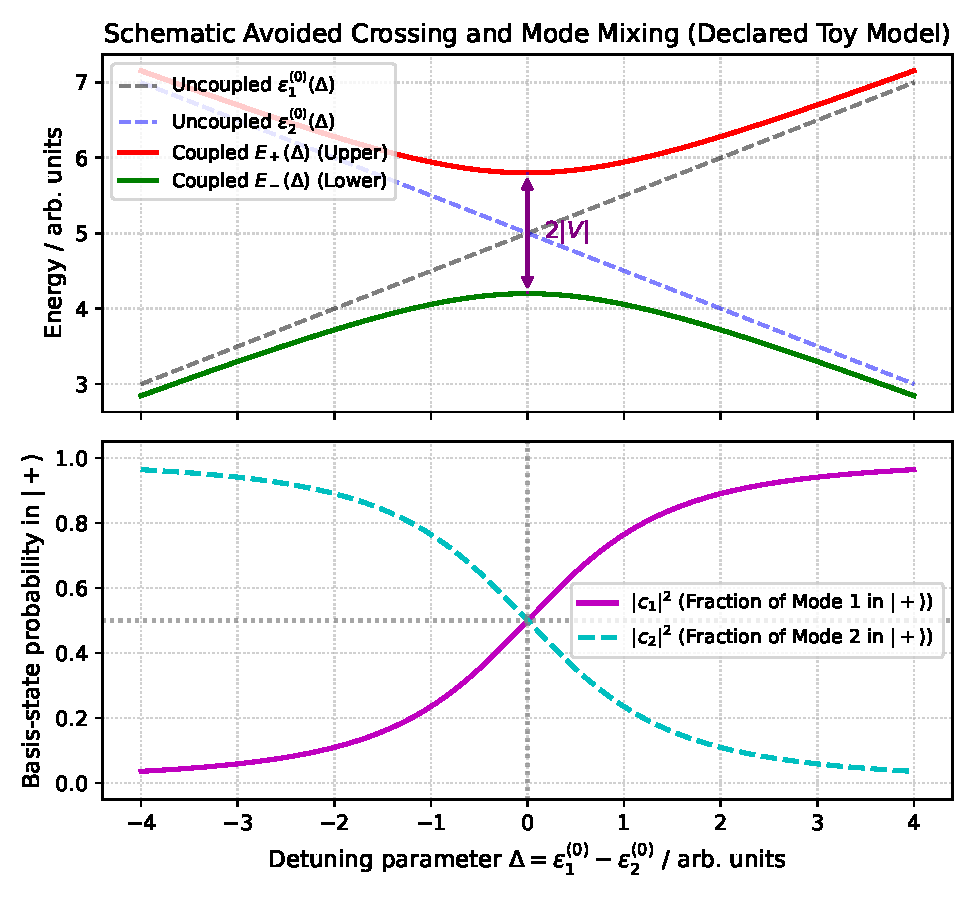
\includegraphics[width=0.95\textwidth]{Img/mode-mixing-avoided-crossing.pdf}
\caption[两态混合的避免交叉与基底概率]{声明参数两态量子混合教学模型中的避免交叉与基底成分权重交换示意图（输入脚本见附录F，采用教学参数 $V=0.8, \bar{\varepsilon}=5.0$ 任意单位）。(a) 未耦合能量本征值（虚线）与耦合后本征能量 $E_\pm(\Delta)$（实线），两支在失谐量 $\Delta = \varepsilon_1^{(0)} - \varepsilon_2^{(0)} = 0$ 处打开能隙 $2V$；(b) 上能级态 $|+\rangle$ 中原始基底 $|1\rangle$（实线）与基底 $|2\rangle$（虚线）的几率权重随失谐量的平滑过渡交换。图示展示的是独立的二态模型数学特性，不代表实核数据。}\label{fig:3-6-mode-mixing}
\end{figure}

联合预言判据包含以下四个相互联系的物理环节：
\begin{enumerate}
\item \textbf{能级避免交叉 (Avoided Crossing)}：随着控制参数改变，未耦合能级可以彼此逼近；在非零耦合作用下，本征能谱不相交。若 $V$ 固定且失谐量穿过零点，最小能隙为 $2V$（见图\ref{fig:3-6-mode-mixing}(a)）；若耦合也随自旋改变，最小间隔的位置和大小要由完整模型计算。
\item \textbf{波函数成分反转与重分布}：穿过避免交叉点前后，高能态与低能态中关于形状振动基底与取向摆动基底的几率成分发生连续交换（见图\ref{fig:3-6-mode-mixing}(b)）。
\item \textbf{电磁跃迁几率的相干干涉与重新分配}：由于电四极算符 $\mathcal{M}(E2)$ 对形状改变和转轴转动态具有不同的跃迁选择定则与矩阵元结构，两态的相干叠加将导致向末态 $|f\rangle$ 的折合跃迁几率展现出特征干涉效应：
\begin{equation}\label{eq:3-6-be2-interference}
B(E2; |+\rangle \to |f\rangle) = \frac{1}{2I_i + 1} \left| \cos\theta\,\langle f || \mathcal{M}(E2) || 1 \rangle + \sin\theta\,\langle f || \mathcal{M}(E2) || 2 \rangle \right|^2 ,
\end{equation}
其中双竖线代表 Wigner--Eckart 约化矩阵元，式前包含初态统计权因子 $\frac{1}{2I_i+1}$。令两个未混合矩阵元为 $M_1,M_2$，交叉项为 $2\cos\theta\sin\theta\,\operatorname{Re}(M_1M_2^*)$；它的大小与符号取决于振幅和相位，也可能为零。相干叠加本身不要求二态子空间覆盖整个希尔伯特空间。在这个固定算符、相同初态自旋的二态旋转中，向同一末态的两个 $B(E2)$ 之和保持不变；把这一性质推广到实核总强度时，还要检查被截去的态和变化的算符。
\item \textbf{多极混合比 $\delta(E2/M1)$ 的演化}：伴随着波函数成分从摆动取向主导向形状振动主导的平滑过渡，带间跨带跃迁的多极混合比 $\delta$ 的数值和符号取决于微观电四极与磁偶极矩阵元的相对相位与干涉效应，并不必然表现为单调显著的变化。
\end{enumerate}

必须强调：单凭实验测得的能级排斥或能级间隔突变，不能唯一确定存在形状模与取向模的耦合。在快转动核结构中，单粒子准粒子顺排（如回弯现象）、带交叉退耦或科里奥利反转均能在能谱上表现为能级排斥。因此，在实验数据分析中，必须严格区分直接谱学测量（能级与分支比）、唯象模型拟合与物理机制解释三层界限。

\subsection{微观自洽响应中旋转赝模的严格剔除}\label{sec:3-6-4}

当在微观准粒子随机相位近似（QRPA）或推转 RPA（CRPA）框架下研究高自旋激发态时，必须处理自发对称破缺引起的零频模问题。\cite{prochniak-rohozinski-2009-bohr-collective-hamiltonian,matsuzaki-2004-nuclear-inertia-and-wobbling}

在旋转参考系中，取推转算符 $\hat H'=\hat H-\omega_{\mathrm{rot}}\hat J_x$，其中 $\hat{\mathbf J}$ 具有作用量量纲，$\omega_{\mathrm{rot}}$ 为角频率。若全哈密顿量满足 $[\hat H,\hat J_k]=0$，角动量代数直接给出
\begin{equation}\label{eq:3-6-rotational-commutators}
[\hat H',\hat J_x]=0,\qquad
[\hat H',\hat J_y\pm i\hat J_z]
=\mp\hbar\omega_{\mathrm{rot}}(\hat J_y\pm i\hat J_z).
\end{equation}
这说明零频方向与推转频率处的转动赝模应区别对待，不能把所有低频解都认作新的形状或摆动激发。破缺平均场加RPA的实现需要检验相应的对称性恢复和赝模解耦。具体模型可以采用经过相容性校准的残余四极力等构造；二次拉伸相互作用是一些实现的选择，并非所有理论必须采用的唯一形式。\cite{matsuzaki-2004-nuclear-inertia-and-wobbling,kvasil-2006-dy156-yb162-crpa-wobbling} 若参考态、残余作用和截断空间不相容，赝模污染便可能影响所求的物理响应。

进一步，微观自洽线性响应导出的有效横向转动响应张量是在参考频率 $\omega_{\mathrm{rot}}$ 的自洽基底上，对小振幅微扰探针角频率 $\Omega$ 导出的动态响应导数：
\begin{equation}\label{eq:3-6-freq-dependent-inertia}
\chi_{kl}^{J\omega}(\Omega; \omega_{\mathrm{rot}}) = \left. \frac{\delta \langle \hat{J}_k \rangle(\Omega)}{\delta \omega_l(\Omega)} \right|_{\omega_{\mathrm{rot}}} .
\end{equation}
该张量依赖探针频率 $\Omega$ 与参考频率 $\omega_{\mathrm{rot}}$，其量纲为转动惯量。怎样从完整响应中构造摆动方程使用的有效横向惯量，取决于模型的约束及赝模处理，不能直接把任意单个张量元命名为通用的 $\mathcal J_\perp$。沿带动力学惯量 $\mathcal{J}^{(2)}=d\langle J_x\rangle/d\omega_{\mathrm{rot}}$ 描述物理角动量对沿带角频率的变化率；若改用无量纲 $I_x=\langle J_x\rangle/\hbar$，右侧需相应乘 $\hbar$。沿带变化与横向取向响应是不同问题。\cite{matsuzaki-2004-nuclear-inertia-and-wobbling}

\subsection{有限自旋非谐效应与局域声子标签边界}\label{sec:3-6-5}

在简谐多声子近似下，摆动带与 $\gamma$ 振动带通常被赋予离散的整数声子量子数 $n_{\mathrm{wob}} = 0, 1, 2, \dots$ 或 $n_\gamma = 0, 1, 2, \dots$。然而，在实际有限核体系中，这种简谐性只是局域展开下的渐近近似。

即使惯量固定，有限角动量也会限制局域声子展开：振幅增大或接近失稳点时，高阶角动量项可能不可忽略。在远离软模、固定低声子数的高自旋展开中，可按 $1/I$ 组织相对修正；这不是所有实核非谐性的统一数值定律。因此，不能把任意三条伴带直接指认为 $n=0,1,2$。不等间隔可能来自有限自旋运动学、准粒子顺排、形状极化或其它混合，需要比较各机制的联合预言。

\subsection{微观模型案例与核区观测边界}\label{sec:3-6-6}

为了审视真实核体系中形状模与取向模耦合的理论预言与实验现状，本小节梳理文献中代表性的微观计算与典型核区的观测边界。

\paragraph{1. TAC-HFB 框架下的高自旋摆动与 $\gamma$ 坐标探索}
Oi 与 Walker 选取 $^{164}\mathrm{Hf}$，用倾斜推转 HFB（TAC-HFB）沿取向角松弛内禀形状，再另设一维示意量子化讨论局域态及其混合。\cite{doctoral-r1-g37-oi-2001-wobbling-gamma-coupling} 这是把形状与取向联系起来的早期模型探索。其HFB空间未重现预期的TSD形变；一维量子化的边界和质量参数也含另外的假设，不能视为完整的微观集体哈密顿量或实验能带。原文以 $a=M_w\omega^2/2$ 定义势能系数后给出的质量关系，还存在反解应保留因子2的代数疑点。这是对原式的一致性核查，尚不足以替代完整模型复算。S/A等局域标记也不应被改称为守恒的实验室空间宇称。

\paragraph{2. 推转 HFB+CRPA 框架下的配对与对顺排响应}
Kvasil 与 Nazmitdinov 用指定的推转 Nilsson 加RPA框架比较 $^{156}\mathrm{Dy}$ 与 $^{162}\mathrm{Yb}$，在模型内将两核的带弯曲分别联系到 $\gamma$ 软化和中子对顺排，并讨论Dy的奇自旋 $\gamma$ 分支向摆动型激发的演化。\cite{kvasil-2006-dy156-yb162-crpa-wobbling} 其配对隙在带交叉附近采用唯象处方；因而“自洽响应”不意味着所有输入均由同一个无近似理论确定。惯量和带间E2/M1的共同比较提供了区分机制的途径，这些仍是该模型范围内的解释。

\paragraph{3. 三轴投影壳模型（TPSM）在偶偶核中的应用与限制}
Bhat 等人用三轴投影壳模型（TPSM），在包含真空、两准粒子及四准粒子构型的截断空间中进行三维角动量投影，比较 $^{76}\mathrm{Ge}, ^{112}\mathrm{Ru}, ^{188,192}\mathrm{Os}, ^{192}\mathrm{Pt}, ^{232}\mathrm{Th}$。\cite{doctoral-r1-g37-bhat-2025-microscopic-wobbling-even-even} 作者结合组态顺排与计算的电磁性质，将其中五个案例解释为摆动型激发，保留 $^{232}\mathrm{Th}$ 为反例。这不等于六核均已获实验确证。轴向形变采用参考输入，非轴形变以再现 $\gamma$ 带头为目标选取，部分配对输入也有调整；拟合所用能量不能再次当作独立验证。需要由寿命、带间电磁强度及其它未参与调参的观测检验这些解释。

形状与取向自由度可以耦合；近简并会放大给定非零相互作用造成的混合，频率不接近也不意味着耦合项必为零。能级排斥只显示相容态间的作用，不能独自辨认被混合的自由度。实际研究应先给出所选模型的能谱、跃迁及响应联合预言，再用未参与调参的资料比较它与准粒子顺排等竞争机制；若现有观测仍不足以区分，就保留这一解释边界。
